\documentclass{imcs}
\usepackage[T2A]{fontenc}
\usepackage[utf8x]{inputenc}
\usepackage[russian]{babel}
\usepackage{graphicx}
\usepackage{hyperref}
\usepackage{enumitem}
\usepackage{listings}
\usepackage{courier}
\usepackage{titlesec}
\usepackage{lscape}
\usepackage{placeins}
\usepackage{tabularx}


\titleformat*{\section}{\LARGE\bfseries\sffamily}
\titleformat*{\subsection}{\Large\bfseries\sffamily}
\titleformat*{\subsubsection}{\large\bfseries\sffamily}
\titleformat*{\paragraph}{\large\bfseries\sffamily}
\titleformat*{\subparagraph}{\large\bfseries\sffamily}

\lstset{basicstyle=\footnotesize\ttfamily,breaklines=true}



\makeatletter
\let\old@itemize=\itemize
\def\itemize{\old@itemize
\setlength{\itemsep}{10pt}
\setlength{\parskip}{0pt}
\setlength{\leftskip}{0pt}
}
\makeatother

\makeatletter
\let\old@enumerate=\enumerate
\def\enumerate{\old@enumerate
\setlength{\itemsep}{10pt}
\setlength{\parskip}{0pt}
\setlength{\leftskip}{0pt}
}\makeatother

\title{Модуль контролируемого исполнения программ Spawner}
\author{Храпченков Пётр Фёдорович}
\mentorinfo{старший преподаватель}
\mentorname{А.С.~Кленин}
\year{2014}



\bibliographystyle{ugost2008}  %% стилевой файл для оформления по ГОСТу
%%%Fixing \thebibliography from eskdbiblist.sty to work with hyperref%%%
%\makeatletter
%\def\thebibliography#1{%
%     \section*{\refname}\phantomsection\addcontentsline{toc}{section}{\refname}%
%      \list{\@biblabel{\@arabic\c@enumiv}}%
%           {\settowidth\labelwidth{\@biblabel{#1}}%
%            \leftmargin\labelwidth
%            \advance\leftmargin\labelsep
%            \@openbib@code
%            \usecounter{enumiv}%
%            \let\p@enumiv\@empty
%            \renewcommand\theenumiv{\@arabic\c@enumiv}}%
%      \sloppy
%      \clubpenalty4000
%      \@clubpenalty \clubpenalty
%      \widowpenalty4000%
%      \sfcode`\.\@m}
%\makeatother
%%%%%%%%%%%%%%%%%%%%%%%%%%%%%%%%%%%%%%%%%%%%%%%%%%%%%%%%%%%%%%%%%%%%


\begin{document}
\maketitle

\tableofcontents
\pagebreak

\section*{Аннотация}
\addcontentsline{toc}{section}{Аннотация}
Модуль Spawner является частью автоматической проверяющей системы CATS и используется для запуска программ с ограничениями на использование системных ресурсов и получения информации об использованных системных ресурсов программой, а так же информации о ходе исполнения.

Рассмотрены подходы к решению проблемы и осуществлена реализация.

\pagebreak

\section{Введение}
\subsection{Глоссарий}

Системные ресурсы -- Набор системных ресурсов включает в себя время исполнения программы в пользовательском режиме, физическое время исполнения, объем выделенной памяти, объем записанной на диск информации.

Физическое время исполнения -- абсолютное время, определяемое глобальным системным таймером.

Уровень загрузки -- величина, отображающая отношение времени в пользовательском режиме к физическому времени.

Время простоя -- время, в течении которого уровень загрузки программы находился не выше установленного минимального.

Механизм песочницы(англ. Sandboxing) -- в компьютерной безопасности защитный механизм для изолированного исполнения программ. Часто используется для запуска непроверенного кода или сомнительных программ от неизвестных разработчиков, поставщиков, подозрительных пользователей или веб сайтов.

JOB\_OBJECT -- это объект, способный иметь имя, настройки безопасности, который контролирует атрибуты ассоциированных с ними процессов. Операции, применяемые к ним, влияют на все процессы, включенные в него. Так, например можно ограничить память, приоритет процессов, а так же завершить их все.


\subsection{Описание предметной области}
\subsubsection{Соревнования по программированию}

На сегодняшний день в России и мире проводится множество соревнований по программированию, включая известный командный чемпионат мира по программированию среди студентов высших учебных заведений АСМ\cite{acm}, а так же олимпиады школьников по информатике.
Подобные соревнования получили широкое распространение и помогают относительно объективно оценить уровень знаний и умений участников в области программирования\cite{prog_challenges}.
В рамках соревнований участникам предлагается набор задач, который они должны решить за определенное время, не выходя за какие-то заданные условиями соревнований ограничения.
Каждому участнику или команде участников предоставляется компьютер с предустановленной средой программного обеспечения, позволяющей сразу же приступить к решению задач.

При проведении соревнования по программированию, от организатора требуется разработать пакет заданий, состоящий как из условий самих задач, так и набора тестов и эталонного решения.
Когда участник разработал программу и считает, что она удовлетворяет условиям задачи, он предоставляет данное решение для проверки организаторам, где, в свою очередь, проходит тестирование и сравнение результата работы программы участника с результатами работы эталонного решения. После этого делается вывод о правильности предложенного на проверку решения.

Для того, чтобы упростить организаторам работу, а участникам их участие, стали применяться так называемые автоматизированные системы организации соревнований. Такие системы обычно состоят из нескольких частей, содержащих в себе интерфейс для наблюдения за ходом соревнования, интерфейс для отправки задач и интерфейс для их проверки. 
%Как правило, разработкой систем организации соревнований так и проведением этих соревнований занимаются университеты.
\FloatBarrier
\subsubsection{Система CATS}

\begin{figure}[htb]
\centering
\includegraphics[width=\textwidth,keepaspectratio]{./img/cats_screenshot.png}
\caption{Веб-интерфейс системы}
\label{cats_screenshot}
\end{figure}

Одной из таких систем является автоматическая система организации соревнований по программированию CATS\cite{cats}\cite{rozhkov}~(Рис.~\ref{cats_screenshot}).
Система разрабатывалась на базе ДВФУ и успешно применяется при проведении соревнований начиная от школьных олимпиад и заканчивая четвертьфиналом чемпионата мира по программированию ACM ICPC.
История системы начинается с 2002 года и продолжается до сих пор.
За это время на базе CATS было проведено огромное количество соревнований, система неоднократно улучшалась и дополнялась\cite{rozhkov}\cite{matvienko}\cite{konovalova}\cite{perepechin}\cite{tuphanov}.
% можно привести список работ связанных с доработкой и улучшением системы %

На текущий момент система включает в себя такие модули как веб-сервер, предоставляющий пользователям веб-интерфейс к CATS, базу данных, а так же модуль judge\cite{rozhkov}(подробнее см. раздел Архитектура).
\subsubsection{Веб-интерфейс}

Веб-интерфейс предоставляет возможность участвовать в доступных турнирах, просматривать задачи, отправлять соответствующие решения, выполненные в разрешенных системой (турниром) средах разработки, следить за ходом их тестирования, следить за ходом турнира и др. Для организаторов, в свою очередь, веб-интерфейс позволяет создавать турниры, добавлять в них задачи, следить за ходом турнира и др.
\FloatBarrier
\subsubsection{База данных}

Связь между веб интерфейсом и модулем judge осуществляется через базу данных.
База данных хранит информацию о существующих в системе турнирах, участниках, задачах, решениях и пр.

Веб интерфейс и база данных являются кросс-платформенными составляющими системы и могут быть установлены на компьютеры под управлением различных операционных систем.

\subsubsection{Модуль judge}

Данный модуль отвечает за самую ответственную часть, иначе говоря за контролируемый запуск и тестирование программ решений участников.
Во время исполнения программ от judge требуется чтобы они не нарушали набора ограничений на системные ресурсы, наборы правил безопасности, а, в случае некорректного хода работы, информация о произошедших ошибках должна быть корректно обработана и учтена.
После чего результаты о ходе тестирования и запуска решения участника отправляются в базу данных.

\subsection{Общая задача контроля исполнения}
В общем случае данная задача является гораздо более обширной, чем будет рассмотрена в рамках данной работы, что, возможно, даст дальнейшее развитие модуля Spawner.
На данный момент уже существует множество менее специфичных инструментов для ее решения.
Для контролируемого исполнения программ используется механизм компьютерной безопасности песочницы\cite{sandboxing_def}.
Песочницы предоставляют жестко контролируемый набор системных ресурсов для заданной исполняемой программы -- например, место на диске, в памяти, время исполнения и пр.
Данная технология находит применение когда требуется исполнить неизвестную программу, которая может содержать потенциально опасный код.
Помимо применения в системах организации соревнований технология получила широкое распространение в современных операционных системах, антивирусах, браузерах и пр\cite{sandboxing_def}.
В общем случае, для создания изолированной среды исполнения требуется большое количество ресурсов, что приводит к большой нагрузке на систему.

В рамках систем проведения соревнований, применение механизма песочницы необходимо для того, чтобы сбои в потенциально содержащих ошибки исполняемых решениях участников не могли привести к сбою системы в целом, а так же чтобы запретить доступ к таким системным ресурсам, как сеть, диск и др.

\subsection{Модуль Spawner}
Для задачи контролируемого исполнения в judge используется модуль Spawner, представленный консольной утилитой\cite{prototype}.
В модуле используются стандартные системные механизмы обеспечения наложения ограничений и создания изолированной среды исполнения.

Через консольный интерфейс задаются накладываемые ограничения а так же опции запуска исполняемой программы.
После исполнения утилитой выдается отчёт, по которому можно получить представление об использовании ресурсов, нарушении ограничений и пр.

Консольный интерфейс был выбран для того, чтобы участники, да и просто все желающие, могли проверять свои решения на предмет соответствия условиям задачи.

До текущего момента модуль Spawner разрабатывался как независимая часть системы CATS и в полной мере отвечал необходимым требованиям.

Однако, консольная утилита Spawner оказалась несовместимой с 64 разрядными операционными системами Windows, в силу специфики программного кода. К тому же, модуль Spawner являясь исполняемым файлом Windows не позволяет проводить более тесную интеграцию веб-сервера с модулем judge из-за отсутствия возможности запуска системно-специфичного кода на других платформах.

К тому же аналогичные модули реализуют более расширенный функционал, например, по вводу дополнительных ограничений, таких как ограничение на время простоя. А вследствие отсутствия финальной версии исходного кода Spawner'а возможность дальнейших изменений и улучшений отсутствует.

Дополнительно, с внедрением новых видов интерактивных задач в соревнования Всероссийской олимпиады школьников по информатике\cite{vseros} появилась необходимость в реализации поддержки таких задач для CATS.
Так же, на базе ДВФУ неоднократно проводились соревнования искусственного интеллекта, где также требуется одновременное контролируемое исполнение программ участников, а так же обмен данными между программами. Эти проблемы привели к постановке задачи множественного исполнения. 

Таким образом, перечисленные выше пункты послужили мотивацией к написанию данной работы.

\subsection{Неформальная постановка задачи}

Требуется доработать модуль Spawner для выполнения следующих требований:
\begin{itemize}
  \item Полная совместимость с предыдущей версией Spawner’а для первоначального внедрения в систему CATS.
  \item Проверка на наличие и корректная обработка исключений, возникших во время работы программы.
  \begin{itemize}
    \item Обработка исключений программы.
    \item Обработка исключений среды разработки.
  \end{itemize}
  \item Ограничения на использование подконтрольной программой системных ресурсов:
  \begin{itemize}
    \item память
    \item время работы
    \item время исполнения
    \item запись в файлы
    \item время простоя
  \end{itemize}
  \item Вывод отчета в других форматах, включая как json, так и форматы отчетов других подобных модулей
  \item Кроссплатформенность
  \begin{itemize}
    \item Возможность работы системы как в 32 так и в 64 битном окружении системы Windows.
    \item Дальнейшая разработка совместимых версий для Linux и др.
  \end{itemize}
  \item Работа со стандартными потоками - stdin, stdout и stderr, их перенаправление
  \item Корректный запуск программ из-под заданного пользователя.
  \item Множественное исполнение программ
  \item Перенаправление потоков ввода вывода
  \item Поддержка ролей запускаемых процессов
  \item Поддержка ролей запускаемых процессов
  \item Анализ и дополнение существующего формата входных аргументов, соответствующего указанным выше требованиям
  \item Интеграция доработок в систему CATS
  \item Возможность отдельного использования функционала утилиты в виде библиотеки.
\end{itemize}


\subsection{Обзор существующих методов решения}

\subsubsection{Существующие решения песочниц}
В настоящее время существует огромное количество доступных механизмов для создания изолированных окружений исполнения программ. Однако не все из них в своем чистом виде удовлетворяют задаче контроля исполнения программ участников соревнований по программированию.
Рассмотрим существующие механизмы песочниц.

\begin{enumerate}
  \item Виртуализация на уровне операционной системы --- использование нескольких изолированных экземпляров пространства пользователя. С точки зрения пользователя эти экземпляры полностью идентичны реальному серверу\cite{virtualization}.
  \item Исполнение, основанное на правилах --- позволяет накладывать ограничения на программы и пользователей, задавая наборы правил для конкретной группы пользователей или программ. Ограничения касаются доступа к файлам, к реестру и т.п. Дополнительно могут использоваться инъекции в код программ, для контроля их поведения.
  \item Виртуальная машина --- полная эмуляция аппаратного обеспечения некоторой платформы. Программы исполняются внутри этого изолированного эмулированного окружения.
  % Добавить Capability Sandbox_(computer_security)
  \item seccomp\cite{seccomp} --- довольно простой, но мощный механизм обеспечения безопасности. Полностью ограничивает работу с системными дескрипторами давая возможность использовать ограниченный набор операций над ними. В случае попытки вызова запрещенных системных функций работа программы будет завершена. Таким образом для программы не создается отдельная виртуальная среда. Вместо этого программа полностью изолируется от системных ресурсов.
\end{enumerate}

Основными критериями в выборе технологии являются: кроссплатформенность, нагрузка на систему, уровень изоляции.

\begin{table}[h!]
\begin{center}
\begin{tabularx}{\textwidth}{|X|c|c|c|X|}
\hline
  Технология &  Кроссплат-  &  Нагрузка  &  Уровень  &  Примеры \\
   &  форменность  &    &  изоляции  &   \\
\hline
 Виртуализация на уровне операционной системы & Да & Средняя & Высокий & chroot, Parallels Virtuozzo Containers, FreeBSD Jail \\
\hline
 Исполнение, основанное на правилах & Нет & Низкая & Средний & SELinux, Apparmor \\
\hline
Виртуальная машина & Да & Высокая & Очень & VirtualBox, VMware \\
  &  &  & высокий & \\
\hline
seccomp & Нет & Низкая & Высокий & --- \\
\hline
Системы проведения соревнований & Да/Нет & Средняя & Средний & spawner, PCMS/Run \\
\hline
\end{tabularx}
\caption{Сравнение технологий песочницы}\label{tab:sandboxing_comparison}
\end{center}
\end{table}
Не смотря на строгие требования к производительности, задача контролируемого исполнения в рамках проведения соревнований по программированию может быть решена одним из указанных способов с высокой изоляцией и нагрузкой на систему. Так, в финале чемпионата мира по программированию ACM активно используется технология виртуальных машин.
Дальнейшее изучение технологии песочниц, возможно, позволит развить данную работу и найти новые способы использования модуля Spawner.
\subsection{Аналогичные модули или системы}

В рамках данной работы было проведено изучение подобных систем организации соревнований по программированию, а так же модулей контролируемого исполнения.
\subsubsection{ejudge}   
ejudge\cite{ejudge} --- это система для проведения различных мероприятий, в которых необходима автоматическая проверка программ. Система может применяться и применяется для проведения олимпиад, поддержки учебных курсов и т.д.
Система предоставляет веб-интерфейс администратора и участника турнира, а так же доступ к серверам турниров из командной строки.
Для контроля исполнения используется патч к ядру Linux. Модуль контроля исполнения программ представляет собой набор скриптов. Невозможно портирование скриптов на ОС Windows в силу их зависимости от системных функций.
\subsubsection{PCMS2/Run}
PCMS2(Programming Contest Management System)\cite{pcms2}
Система контроля исполнения представляет собой консольную утилиту. В программе используется динамическая библиотека с вынесенными функциями.
Используется во время проведения Всероссийского этапа ACM ICPC.
Для контролируемого исполнения постоянно использует режим отладки.
Также следует отметить, что присутствует возможность создания и контроля исполнения процесса от другого пользователя, но для этого требуются особые привилегии.
\subsubsection{Contester}
Contester\cite{contester} --- это система для проведения турниров и индивидуального решения задач по олимпиадному программированию (спортивному программированию). Система содержит условия задач - от легких до олимпиадных - и возможность проверки решений на большинстве современных языков: C++, Object Pascal, Java и языках .NET: C\#, J\# и Visual Basic.

Contester работает на Windows и на Linux. Язык реализации Delphi/freepascal. Представляет собой полноценную систему организации соревнований готовую к запуску с момента установки и распространяется в виде установочного файла или архива, в зависимости от операционной системы.
% Нужно изучить подробнее!!! %
\subsubsection{Executor}
Executor\cite{executor} --- автоматизированная сетевая тестирующая система для проведения турниров по программированию по правилам ACM. Executor - freeware, распространяется бесплатно и без каких-либо ограничений на использование.
Тестирование контроля исполнения не производилось, так как сайт не работает (домен зарегестрирован на localhost).
\subsubsection{PC$^2$}
PC$^2$(Programming Contest Control System)\cite{pccs} --- система разработанная в Калифорнийском Государственном Университете Sacramento (CSUS) в поддержку соревнований по программированию, проводимых ACM и, в частности, ACM International Collegiate Programming Contest (ICPC) и его региональных этапов. 
Контроль исполнения, как неотъемлемая часть общей системы.
\subsubsection{olympiads.ru/RUN}
Система самотестирования olympiads.ru\cite{olympiads}. Используется для тестирования решений задач, представленных на соответствующем сайте. Система работает на платформе Windows, имеет инсталляционную программу и документацию. Не умеет компилировать, проверяет только exe, непригодна для проведения соревнований.
Вследствие того что система не поддерживается с 2003 года и имеет узкий функционал в рамках данной работы детально рассматриваться не будет.
\subsubsection{DOMjudge}
DOMjudge\cite{domjudge} --- автоматизированная тестирующая система, для проведения соревнований по программированию, подобных ACM ICPC. Основной упор сделан на удобство использования и безопасность. Система применялась во многих соревнованиях, распространяется свободно на условиях открытого ПО. 
Для контроля исполнения используется набор небольших консольных утилит.
\subsubsection{dudge}
Dudge\cite{dudge} --- это универсальная система для проведения олимпиад по программированию и другим предметам, написанная на Java и J2EE с использованием СУБД PostgresSQL и распространяющаяся по лицензии GPL. 
В качестве контроля исполнения используется динамическая библиотека, реализована для Windows и Unix. Библиотека используется в Java коде. Для создания и контроля исполнения процесса от другого пользователя требуются особые привилегии.%(не подтверждено)%
\subsubsection{openjudge/sandbox}
openjudge/sandbox\cite{openjudge} --- набор библиотек, предоставляющий API, которое можно использовать для контроля простых программ с единственным процессом в ограниченном окружении, или, говоря иначе, песочнице. Позволяет создавать инструменты которые могут отслеживать и блокировать поведение исполняемых программ прямо во время исполнения.

Простая в обращении библиотека. Возможно использование для портирования под Linux.
\subsubsection{CATS/Spawner 1}
CATS\cite{prototype} --- автоматизированная тестирующая система, для проведения как одиночных, так и командных соревнований по программированию.
Для контроля исполнения используется консольная утилита. Создание и контроль исполнения процесса от другого пользователя требуют особые привилегии. Не поддерживается.
\subsubsection{Spawner 2}
Дальнейшее развитие модуля контроля запуска и исполнения программ cats-judge/Spawner\cite{spawner_src}.
На данный момент представляет собой обратно совместимую консольную утилиту с дополненными и улучшенными, по сравнению с предыдущей версией, возможностями.
Функционал реализован только для систем семейства Windows.

\begin{landscape}
\begin{table}[h!]
\begin{center}
\begin{tabularx}{25cm}{|X|X|X|X|X|X|X|}
\hline
  Название   &  Операционная система  &  Лицензия  &  Интерфейс  &  Язык	реализации 		&  Запуск под другим	пользователем  & Комментарий \\
\hline
ejudge  &  Linux          &  GPL        &    Набор утилит         &  С          &  ?   &   ---    \\% так ли это
\hline
PCMS2/Run &  Windows  & Открытый код        &     Консольная утилита + динамич библиотека  &  С++          &  + права  &   Аналогична спавнеру    \\
\hline
Contester &  ?          &  ?        &   ?          &  ?          &  ?   &   ---    \\
\hline
Executor &  Windows 2000/XP/2003          &  Закрытый код        &   ?          &  ?          &  ?   &   ---    \\
\hline
PC$^2$ &  Windows, Linux          &  Закрытый код        &             &  +          &  +   &   ---  \\
\hline
olympiads.ru/ RUN &  Windows          &  Закрытый код        &   Исполняемый файл          &  ?          &  -   &   ---    \\
\hline
DOMjudge &     Linux      &  GPL\cite{gpl}       &      Набор консольных утилит       &  C          &  -   &   Запись статусов в файлы    \\
\hline
dudge &  Windows, Unix          &  GPL        &     Динамич. библиотека + биндинг        &  С/Java          &  ?   &   ---    \\
\hline
openjudge/ sandbox &  Linux          &  Закрытый код        &    Библиотека         &  C          &  ?   &       \\
\hline
CATS/ Spawner1 &  Windows x86          &  ???        &    Консольная утилита         &  C          &  + права  &   ---    \\
\hline
Spawner2 &  Windows          &  GPL        &     Консольная утилита        &  C++          &  +   &   ---    \\
\hline
\end{tabularx}
\caption{Сравнение доступных систем контроля исполнения программ}\label{tab:wsi_diff_rel}
\end{center}
\end{table}
\end{landscape}

По полученным данным можно судить о том что большинство популярных систем либо имеют закрытый код, либо являются платформозависимыми. Так же нельзя не отметить простоту библиотеки sandbox. В рамках данной работы для реализации функционала контролируемого исполнения под системами Linux предлагается использовать именно её.


\subsubsection{Описание предшествующих работ}
Студенты нашей кафедры успешно развивали систему CATS и модуль Spawner:
\begin{enumerate}

    \item Дипломная работа «Система автоматического тестирования программ и организации соревнований по программированию», Автор Рожков М. Руководитель Кленин А. С. 2004\cite{rozhkov}
    \item Курсовая работа «Рендеринг математических выражений в MathML и HTML», Автор Матвиенко В. Руководитель Кленин А. С. 2005\cite{matvienko}
    \item Курсовая работа «Поиск сходных алгоритмических конструкций в программном коде», Автор Коновалова Д. Руководитель Кленин А. С. 2005\cite{konovalova}
    \item Курсовая работа «AJAX-интерфейс для системы CATS», Автор Перепечин В.В. Руководитель Кленин А. С. 2007\cite{perepechin}
    \item Курсовая работа «Универсальный генератор тестов для системы CATS», Автор Туфанов И.Е. Руководитель Кленин А. С. 2008\cite{tuphanov}
    \item Курсовая работа «Модуль контролируемого исполнения программ Spawner», Автор Храпченков П.Ф. Руководитель Кленин А. С. 2013\cite{khrapchenkov}
\end{enumerate}

\subsubsection{Вывод}

Ценность данной работы подтверждается неугасающей популярностью соревнований по программированию и, как следствие, необходимостью развивать уже существующую систему CATS в целом и модуль Spawner в частности. 

\subsection{План работ}

\begin{enumerate}
    \item Рассмотреть возможность улучшения взаимодействия модуля judge со Spawner'ом.
    \item Рассмотреть возможность переработки процедуры парсинга командных аргументов.
      \begin{itemize}
          \item Изучить существующий набор опций и аргументов и оптимизировать его.
          \item Добавить возможность изменять набор консольных аргументов.
      \end{itemize}        
    \item Изучить готовые решения sandboxing'а.
    \item Изучить openjudge/sandbox.
    \item Спроектировать реализацию.
    \item Поэтапно осуществить реализацию:
      \begin{itemize}
          \item Реализовать улучшенное взаимодействие с judge.
          \item Пересмотреть набор консольных аргументов и переписать их парсер.
          \item Добавить поддержку openjudge/sandbox.
      \end{itemize}        
\end{enumerate}

\section{Требования к окружению}

\subsection{Требования к аппаратному обеспечению}

Для работы требуется компьютер, пригодный для компиляции исходного кода программы или исполнения существующих пакетов.
Т.е. кроме работающих процессора, оперативной и постоянной памяти требуются
клавиатура и монитор.

\subsection{Требования к программному обеспечению}

\subsubsection{Для разработчика}
\begin{itemize}
  \item ОС Windows не ниже XP
  \item CMake не ниже 2.6
  \item Компилятор C++(MSVC++ 2005+) или g++ 4.7.7 и выше
  \item Perl 5 для тестов
  \item Необходимые компиляторы и интерпретаторы для языков тестовых программ
\end{itemize}
\subsubsection{Для пользователя}
\begin{itemize}
  \item ОС Windows не ниже XP
  \item При необходимости запуска процессов от имени другого пользователя - учетная запись с ограничениями
\end{itemize}
    
\subsection{Требования к пользователям}
От пользователей требуется умение пользоваться консолью.

\section{Архитектура системы}

Несмотря на то, что для конечного пользователя автоматизированная система представлена в виде Web интерфейса, она является аппаратно-програмным комплексом, состоящим из нескольких модулей.
В рамках данной работы необходимо рассмотреть внутреннее устройство системы, для обоснования некоторых принятых решений.
\iffalse TODO: каких? \fi

\subsection{Архитектура системы CATS}
Автоматизированная система CATS состоит из нескольких частей: веб-интерфейс, база данных, а так же модуль judge. 


\subsubsection{Веб-интерфейс}
Веб-интерфейс\cite{rozhkov} является кросс-платформенной частью системы. Веб сервер может быть запущен практически на любой системе.
Фактически, с помощью веб-интерфейса осуществляется управление содержимым базы данных. 

\subsubsection{База данных}
\FloatBarrier
В базе данных\cite{rozhkov} системы хранятся данные о проводимых турнирах, пакеты задач, исходный код, информация об участниках, их попытках, а так же информация по средам разработки.
Однако привязка модуля judge к какому-либо виду базы данных усложняет его развертывание на конечной машине.

\begin{figure}[htb]
\centering
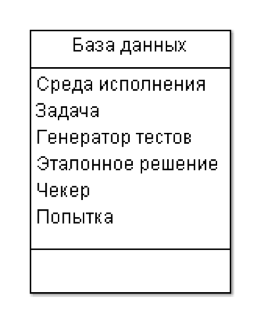
\includegraphics{./img/db.png}
\caption{Схематичное изображение базы данных}
\label{dbfields}
\end{figure}

\FloatBarrier
\subsubsection{Модуль judge}
\FloatBarrier
Модуль judge\cite{rozhkov} в свою очередь содержит загруженный кэш задач, кэш попыток, различные конфигурационные файлы и модуль Spawner.

Обычно, для сокращения нагрузки одновременно запущено несколько компьютеров с judge. Они подключаются к базе данных и распределяют задачи на исполнение между собой.

\begin{figure}[htb]
\centering
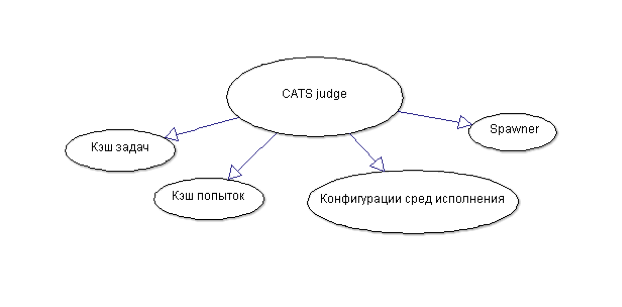
\includegraphics{./img/judge.png}
\caption{Схематичное устройство модуля judge}
\label{judgemodule}
\end{figure}

\FloatBarrier
В случае отсутствия задачи в кэше происходит загрузка из базы данных, генерация тестов и т.д.

В общем случае коммуникация между модулями проходит в следующем порядке:

\FloatBarrier
\begin{figure}[htb]
\centering
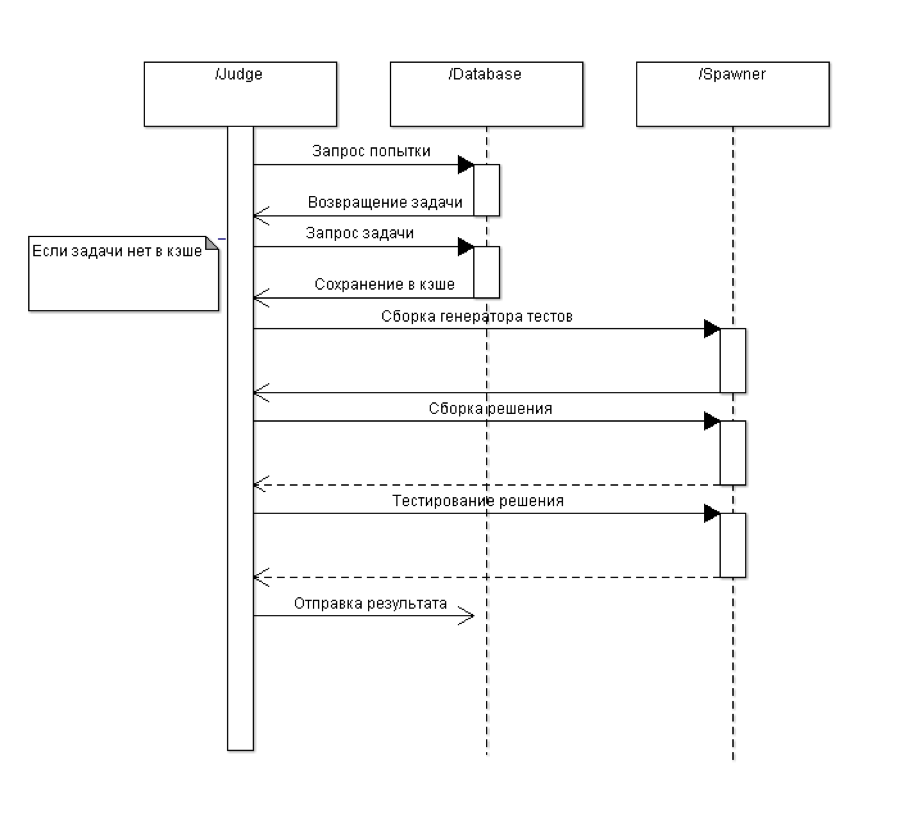
\includegraphics{./img/judgeinteraction.png}
\caption{Схема работы модуля judge}
\label{judgeinteraction}
\end{figure}

\FloatBarrier
\subsubsection{Модуль Spawner}

Во время проведения тестирования требуется создать для программы достаточно изолированную среду и задать необходимые ограничения на ресурсы. Так же в случае некорректного хода исполнения тестируемой программы требуется определить характер и возможную причину ошибок и должным образом отреагировать на это. Этой работой занимается модуль Spawner.

\FloatBarrier 
Являясь подмодулем judge, Spawner в свою очередь разбит на три основных слоя: консольный интерфейс, прослойка совместимости и библиотека с набором внутренних классов.
\begin{figure}[htb]
\centering
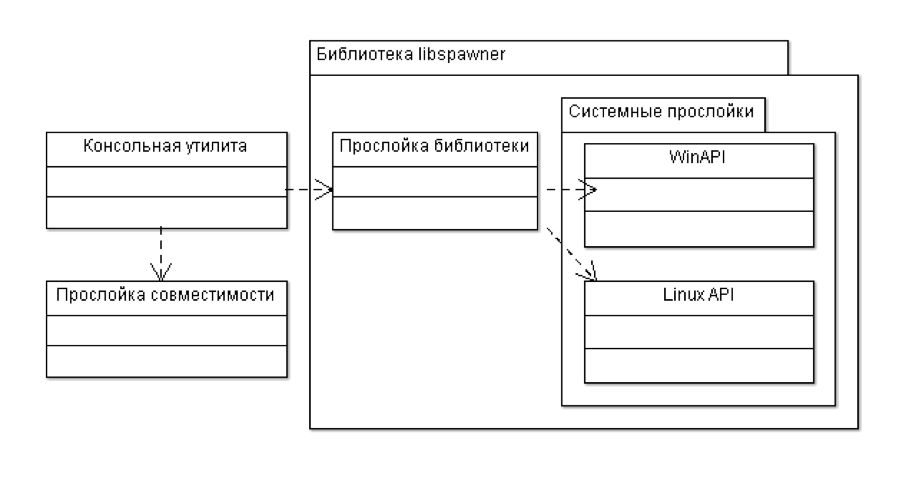
\includegraphics{./img/sp.png}
\caption{Схема устройства модуля Spawner}
\label{spawnermodule}
\end{figure}
\FloatBarrier
Консольная утилита предоставляет интерфейс командной строки пользователю и, в зависимости от режима совместимости, набор аргументов и формат отчета.
Режим совместимости задается специальным параметром.
Прослойка совместимости выполняет связующую роль выходных данных библиотеки libspawner и требуемого формата отчета/аргументов.
Сама же библиотека представляет набор интерфейсов, обеспечивающий доступ к конечным функциям операционной системы.

На текущий момент

\section{Спецификация данных}
\subsection{Ограничения}
Любые неправильные значения перечисленных ниже ограничений(например строковые константы) приводят к игнорированию соответствующего аргумента.
Ограничения можно задавать и в других смежных единицах, так например память можно указывать в килобайтах(kB), а время в минутах (m). Подробнее смотри соответствующий раздел.
По превышению любого из ограничений программа завершается с соответсвующим статусом. Иначе программа завершается со статусом ExitProcess.

\begin{landscape}
\begin{table}[h!]
\begin{center}
\begin{tabularx}{25cm}{|X|c|X|X|c|X|}
\hline
  Ограничение & Опция  &  Переменная  &  Статус & Единицы & Описание\\
   & & окружения  &  по заершению &  & \\
\hline
  Время в пользовательском режиме & -tl & SP\_TIME\_LIMIT & TimeLimitExceeded & секунды & Устанавливает ограничение на время исполнения процесса в пользовательском режиме\\
\hline
  Фактическое время & -d & SP\_DEADLINE & TimeLimitExceeded & мегабайты & Устанавливает ограничение на физическое время исполнения программы\\
\hline
  Память & -tl & SP\_MEMORY  & MemoryLimitExceeded & мегабайты & Устанавливает ограничение на используемую память\\
\hline
  Жесткий диск & -tl & SP\_WRITE\_LIMIT & WriteLimitExceeded & мегабайты & Устанавливает ограничение на запись в файл\\
\hline
  Минимальный уровень загрузки & -tl & SP\_LOAD & --- & проценты & Устанавливает минимальный порог уровня загрузки.\\
\hline
  Время простоя & -lr & SP\_IDLE\_LIMIT & IdleLimitExceeded & секунды & Устанавливает ограничение на время в состоянии простоя.\\
\hline
  Ограничение на системные ресурсы & -s & SP\_SECURITY & & & Устанавливает ограничение на работу с системными дескрипторами \\
\hline
\end{tabularx}
\caption{Ограничения Spawner'a}\label{tab:sp_rest}
\end{center}
\end{table}
\end{landscape}


\paragraph{Перевод единиц измерения}
Поддерживаются единицы трех видов – память, время и безтиповые. У памяти основными единицами являются байт и бит, у времени – секунда, минута, час, день.

\begin{table}[h!]
\begin{center}
\begin{tabular}{|l|c|l|}
\hline
Единица & Тип & Краткая запись\\
\hline
Байт & Память & B\\
\hline
Бит & Память & b\\
\hline
Секунда & Время &s\\
\hline
Минута  & Время &  m\\
\hline
Час & Время  & h\\
\hline
День &  Время & d\\
\hline
\end{tabular}
\caption{Единицы измерения}\label{tab:sp_units}
\end{center}
\end{table}

Так же возможно добавление префикса из системы «Си». Т.е. например – мегабайт, килобит, миллисекунда и т.д.

\begin{table}[h!]
\begin{center}
\begin{tabular}{|l|c|l|}
\hline
Префикс & Значение &  Краткая запись\\
\hline
Дека &  10  & da\\
\hline
Гекто & $10^2$  & h\\
\hline
Кило - Киби & $10^3$ - $1024^1$ & k - Ki\\
\hline
Мега - Меби & $10^6$ - $1024^2$ & M - Mi\\
\hline
Гига - Гиби & $10^9$ - $1024^3$ & G - Gi\\
\hline
Тера - Теби & $10^{12}$ - $1024^4$  & T - Ti\\
\hline
Деци  & $10^{-1}$ & d\\
\hline
Санти & $10^{-2}$ & c\\
\hline
Милли & $10^{-3}$ & m\\
\hline
Микро & $10^{-6}$ & u\\
\hline
\end{tabular}
\caption{Степени единиц измерения}\label{tab:sp_degrees}
\end{center}
\end{table}

Таким образом, значение ограничения можно записывать в виде: 
\begin{lstlisting}
<value>[degree][unit]
\end{lstlisting}
Где value -- значение, degree -- степень, unit -- единица измерения.
Если указано только значение, то его единица измерения будет установлена по-умолчанию.
 
\subsection{Опции общие для всех режимов совместимости}
\subsubsection{Выбор режима совместимости}

Ключ -- - -legacy=<значение>

Переменная окружения -- SP\_LEGACY = <значение>

Возможные значения -- sp99, sp00, pcms2

sp99 -- режим совместимости со старой версией Spawner'а.
 
sp00 -- основной режим Spawner'а.

pcms2 -- режим совместимости с PCMS2/Run
\subsubsection{Вывод помощи}

Ключ -- - -help, -h

Выводит справку для конкретно выбранного режима совместимости

\subsection{Опции Spawner}
\paragraph{Отключение системных диалогов ошибок}
Задается ключом -- - -hide\_errors

Отключает стандартный диалог о составлении отчета об ошибке, а так же диалог исключения. Подробнее смотри соответствующий раздел.

\paragraph{Отключение отображения пользовательского интерфейса}
Задается ключом -- - -hide\_gui

Отключает видимый пользовательский интерфейс и окна. Подробнее смотри соответствующий раздел.

\paragraph{Отключение ошибок crtdebug}
Задается ключом -- - -hide\_crt

Отключает у программ, скомпилированных в Visual Studio в конфигурации Debug отображение окна исключения crtdebug. Подробнее смотри соответствующий раздел.

\paragraph{Запуск программы с поиском ее в системных путях}
Задается ключом -- - -systempath

Позволяет системе искать исполняемый файл запускаемой программы в системных путях.

\paragraph{Рабочая директория}
Задается ключом -wd=<working\_directory>

Устанавливает рабочую директорию для запускаемой программы.

\paragraph{Управление стандартным потоком ввода процесса}
Задается ключом -- - -in=<what>

Перенаправляет поток ввода исполняемого процесса на указанный ресурс. Если <what> начинается с *, то будет произведен поиск по глобальному пространству имен, в которое входят идентификаторы stdout, stdin, stderr, report, и произведено соответствующее соединение или будет выдан отчет с ошибкой.

Переменная окружения   SP\_INPUT\_FILE

\paragraph{Управление стандартным потоком вывода процесса}
Задается ключом -- - -out=<what>

Перенаправляет поток вывода исполняемого процесса на указанный ресурс. Если <what> начинается с *, то будет произведен поиск по глобальному пространству имен, в которое входят идентификаторы stdout, stdin, stderr, report, и произведено соответствующее соединение или будет выдан отчет с ошибкой.

Переменная окружения   SP\_OUTPUT\_FILE

\paragraph{Управление стандартным потоком ошибок процесса}
Задается ключом -- - -err=<what>

Перенаправляет поток ошибок исполняемого процесса на указанный ресурс. Если <what> начинается с *, то будет произведен поиск по глобальному пространству имен, в которое входят идентификаторы stdout, stdin, stderr, report, и произведено соответствующее соединение или будет выдан отчет с ошибкой.

Переменная окружения   SP\_ERROR\_FILE

\paragraph{Установка имени пользователя}
Задается ключом -- -u=user@domain

Устанавливает имя пользователя для делегированного запуска программы. Работает только в связке с опцией пароля - -p=<password>. 

Переменная окружения   SP\_USER

\paragraph{Установка пароля пользователя}
Задается ключом  -- -p=<password>

Устанавливает пароль для делегированного запуска программы. Работает только в связке с опцией пароля - -u=user@domain. 

Переменная окружения   SP\_PASSWORD

%\paragraph{ФОРМАТ ОТЧЕТА}
%Задается ключом --report\_format=<format>

%Задает формат отчета. На текущий момент дополнительно стандартному отчету доступен отчет в формате json.

%Переменная окружения   SP\_REPORT\_FORMAT

\subsection{Опции для совместимости с предыдущей версией Spawner'a}
\paragraph{Совпадающие опции}
Совпадающие опции имеют абсолютно тот же функционал с новым стандартом Spawner’а
\begin{table}[h!]
\begin{center}
\begin{tabular}{|l|c|}
\hline
Опция старой версии & Опция новой версии\\
\hline
–i:<what> & - -in=<what>\\
\hline
–so:<what> &  - -out=<what>\\
\hline
–se:<what> & - -err=<what>\\
\hline
\end{tabular}
\end{center}
\end{table}

\subsubsection{Сохранение отчета в файл}
Задается ключом -- –sr:<what>

Сохраняет сгенерированный отчет в заданный файл. 

Переменная окружения   SP\_REPORT\_FILE

\subsubsection{Скрыть отчет}
Задается ключом -- –hr:<what>

Если значение опции 1, то возвращаемый отчет не выводится.

Переменная окружения   SP\_HIDE\_REPORT

\subsubsection{Скрыть стандартный вывод приложения}
Задается ключом -- –ho:<what>

Если значение опции 1, то возвращаемый программой стандартный вывод не выводится в консоль.

Переменная окружения   SP\_HIDE\_OUTPUT
\subsection{Опции совместимости с PCMS2/Run}
{Ограничения}
\subsubsection{Ограничение времени в пользовательском режиме}

Ключ -- -t <значение>

Задает ограничение на время исполнения в пользовательском режиме. Единицы по-умолчанию секунды.
\subsubsection{Ограничение оперативной памяти}

Ключ -- -m <значение>

Задает ограничение на оперативную память. Единицы по-умолчанию мегабайты.
\subsubsection{Минимальный порог загрузки}

Ключ -- -r <значение>

Задает порог загрузки для определения состояния простоя. По-умолчанию принимает дробные значения от 0 до 1. Может принимать значения выраженные в процентах, например 25\%.
\subsubsection{Ограничение на время простоя}

Ключ -- -y <значение>

Задает ограничение на время исполнения в состоянии простоя. Единицы по-умолчанию секунды.
\subsubsection{Другие опции}
\begin{table}[h!]
\begin{center}
\begin{tabular}{|l|c|}
\hline
Название & Ключ\\
\hline
Имя пользователя & -l <значение>\\
\hline
Пароль & -p <значение>\\
\hline
Рабочая директория & -d <значение>\\
\hline
Сохранить отчет в файл & -s <значение>\\
\hline
Сохранить stdout в файл & -o <значение>\\
\hline
Сохранить stderr в файл & -e <значение>\\
\hline
Считать stdin из файла & -i <значение>\\
\hline
Не выводить в консоль & -q\\
\hline
Показать интерфейс & -w\\
\hline
\end{tabular}
\end{center}
\end{table}
\subsection{Формат отчета}
\subsubsection{Отчет модуля Spawner1}
По завершению работы контролируемого процесса в консоль и/или в выбранный файл выводится отформатированный отчет.
Все значения выводятся в виде

<Свойство>:   <Значение>\[ Единица измерения\]
В первой половине отчета идет описание заданных ограничений и опций, а во второй - рабочие значения по соответствующим характеристикам, а так же статусы.

Пример совместимой версии отчета:
\begin{lstlisting}
spawner>sp --cmd gcc.exe

--------------- Spawner report ---------------
Application:               gcc.exe
Parameters:                <none>
SecurityLevel:             0
CreateProcessMethod:       CreateProcess
UserName:                  shigidono
UserTimeLimit:             Infinity
Deadline:                  Infinity
MemoryLimit:               Infinity
WriteLimit:                Infinity
----------------------------------------------
UserTime:                  0.000000 (sec)
PeakMemoryUsed:            0.953125 (Mb)
Written:                   0.000060 (Mb)
TerminateReason:           ExitProcess
ExitStatus:                1
----------------------------------------------
SpawnerError:              <none>
\end{lstlisting}

И для предыдущей версии spawner’а
\begin{lstlisting}
sp gcc.exe

--------------- Spawner report ---------------
Application:           gcc.exe
Parameters:            <none>
SecurityLevel:         0
CreateProcessMethod:   CreateProcess
UserName:              shigidono
UserTimeLimit:         Infinity
DeadLine:              Infinity
MemoryLimit:           Infinity
WriteLimit:            Infinity
----------------------------------------------
UserTime:              0.000000 (sec)
PeakMemoryUsed:        0.000000 (Mb)
Written:               0.000000 (Mb)
TerminateReason:       <none>
ExitStatus:            0
----------------------------------------------
SpawnerError:          CreateProcess failed with error 2 ()
\end{lstlisting}

В данном формате отчета:
\begin{itemize}
  \item Application - Имя приложения;
  \item Parameters - Параметры приложения;
  \item SecurityLevel - Уровень защиты;
  \item CreateProcessMethod – Метод создания процесса;
  \item UserName - Имя пользователя под которым был запущен дочерний процесс в формате: User[@Domain];
  \item UserTimeLimit - максимальное время в сек. выполнения процесса в пользовательском режиме по истечении  которого процесс прерывается. По умолчанию: "Infinity";
  \item Deadline - Время в сек., которое выделено процессу. По умолчанию: "Infinity";
  \item Отличается от TimeLimit тем, что это физическое время. Если процесс непрерывно осуществляет ввод/вывод, находиться в состоянии ожидания или система перегружена,  то процесс может выполнятся неограниченно долго несмотря на TimeLimit. Для предотвращения данной ситуации нужно установить DeadLine;
  \item MemoryLimit - Максимальный объем выдаляемой памяти процессу в Mb. По умолчанию: "Infinity";
  \item WriteLimit - Максимальный объем информации, который может быть записан процессом в Mb. По умолчанию: "Infinity";
  \item UserTime - Фактическое время выполнения процесса в сек;
  \item PeakMemoryUsed - Максимальное использование виртуальной памяти процессом в Mb;
  \item Written - Объем информации, который был записан процессом в Mb;
  \item TerminateReason - Причина завершения процесса. Может быть:  
  \begin{itemize}       
    \item "ExitProcess"\, -- процесс завершился нормально
    \item "MemoryLimitExceeded"\, -- превышен лимит памяти
    \item "TimeLimitExceeded"\, -- превышен лимит времени выполнения (либо TimeLimit, либо Deadline);
    \item "WriteLimitExceeded"\, -- превышен лимит записи;
    \item "AbormalExitProcess"\, -- процесс завершился с исключением (список исключений см. ниже);
  \end{itemize}
  Если процесс не был завершен, то данному полю соответствует значение "\,<none>".                
  \item ExitStatus - Статус завершения процесса. Принимает значение кода возврата процесса. Если ExitStatus = 0, то процесс завершился нормально.
  \item SpawnerError - Текст ошибки при работе Spawner'а. Если при работе ошибка не произошла, то полю соотвествует значение "\,<none>".
\end{itemize}
\subsubsection{Отчет в режиме совместимости с PCMS2/Run}
В результате исполнения модуля в режиме совместимости pcms2 и в случае, когда не отключен вывод на консоль, выводится следующий отчет:
\begin{lstlisting}
Running "c:\Windows\System32\PING.EXE ya.ru", press ESC to terminate...
Memory limit exceeded
Program tried to allocate more than 10 bytes
  time consumed: 0.00 of 1.00 sec
  time passed:   0.03 sec
  peak memory:   155648 of 10 bytes
\end{lstlisting}
Когда задан файл для вывода отчета, отчет выводится в следующем формате:
\begin{lstlisting}
average.memoryConsumed=1125376.000
average.timeConsumed=15.250
average.timePassed=446.000
invocations=4
last.memoryConsumed=155648
last.timeConsumed=0
last.timePassed=30
max.memoryConsumed=4030464
max.timeConsumed=46
max.timePassed=1518
min.memoryConsumed=155648
min.timeConsumed=0
min.timePassed=30
total.memoryConsumed=4501504
total.timeConsumed=61
total.timePassed=1784
\end{lstlisting}


\subsubsection{Отчет Json}
Для простоты более плотной интеграции с другими модулями, такими как judge было принято решение о реализации вывода отчета в формате json. Вывод в этом формате задается специальным аргументом или переменной окружения.
Пример отчета:
\begin{lstlisting}
{
   "Application" : "3.exe",
   "CreateProcessMethod" : "CreateProcess",
   "Deadline" : "Infinity",
   "ExitCode" : 0,
   "ExitStatus" : "0",
   "MemoryLimit" : {
      "real_value" : 268435456,
      "units" : "MB",
      "value" : 256.0
   },
   "Parameters" : [],
   "PeakMemoryUsed" : {
      "real_value" : 0,
      "units" : "MB",
      "value" : 0.0
   },
   "SecurityLevel" : false,
   "SpawnerError" : "<none>",
   "TerminateReason" : "MemoryLimitExceeded",
   "UserName" : "shigidono",
   "UserTime" : {
      "real_value" : 0,
      "units" : "Second",
      "value" : 0.0
   },
   "UserTimeLimit" : {
      "real_value" : 1000,
      "units" : "Second",
      "value" : 1.0
   },
   "WriteLimit" : {
      "real_value" : 31457280,
      "units" : "MB",
      "value" : 30.0
   },
   "Written" : {
      "real_value" : 0,
      "units" : "MB",
      "value" : 0.0
   }
}
\end{lstlisting}

\subsection{Множественный ввод/вывод}
Благодаря своей структуре, библиотека libspawner позволяет сделать множественное определение потоков вывода. Так поток вывода программы может быть направлен как на стандартный вывод в консоль, так на запись в файл. Эти процессы происходят одновременно. Возможно это благодаря тому, что каждому потоку вывода можно сопоставить несколько конечных и начальных точек.
В консоли это решается путем задания соответствующих конкретным потокам вывода аргументов.
Например:
\begin{lstlisting}
sp.exe --out=1.txt --out=2.txt --out=*std a.exe
\end{lstlisting}
Данная команда произведет запись в 2 файла и выведет информацию со стандартного потока вывода программы а.ехе в консоль.
\subsection{Запуск многих процессов}
В данной работе был спроектирован и реализован консольный интерфейс запуска многих процессов.
Для разделения аргументов, опций и ограничений, принадлежащих разным программам, используется специальный ключ-разделитель. Он задается при помощи флага 
\begin{lstlisting}
--separator=<separator_string>
\end{lstlisting}
После этого когда в аргументах Spawner’а встречается флаг вида - -<separator\_string>, система считает следующий за ним набор аргументов принадлежащих следующей программе. В случае если внутри двух флагов разделителей не встречаются аргументы необходимые для запуска программы, Spawner выдает отчет с ошибкой.
Для перенаправления портов ввода/вывода используется синтаксис ссылок и пространств имен. Каждая программа представляется в виде пространства имен с идентификатором, по умолчанию являющимся порядковым номером программы от 0. Каждое пространство имен предоставляет такие идентификаторы, как stdout, stderr, stdin, report. Т.е. для того чтобы подключить к потоку ввода поток вывода 2го процесса необходимо задать следующий флаг
\begin{lstlisting}
--in:*1.stdout
\end{lstlisting}

Пример
\begin{lstlisting}
sp.exe --separator=// --in:*1.stdout program.exe --// --in:*0.stdout --err:error.txt checker.exe --// --in:*0.stderr logger.exe
\end{lstlisting}
В данном примере поток вывода 2го процесса будет подключен к потоку ввода первого, а поток вывода первого процесса – ко вводу второго.
Можно изменить идентификатор программы внутри пространства аргументов этой программы, задав флаг –program:<id>, причем <id> не может содержать служебные символы. Тогда обращение будет выглядеть как - -in:*<id>.stdout

\pagebreak



\section{Функциональные требования}
Spawner должен соответствовать следующим требованиям
\begin{enumerate}
    \item Возможность накладывать ограничения:
        \begin{itemize}
            \item Ограничение на объем памяти используемой исполняемой программой
            \item Ограничение на объем дискового пространства доступного исполняемой программе
            \item Ограничение на время исполнения в пользовательском режиме ОС
            \item Ограничение на фактическое время исполнения
            \item Ограничение на время простоя вместе с ограничением на пороговое значение загрузки
            \item Ограничение на доступ к системным дескрипторам
        \end{itemize}
    \item Корректная обработка ошибок:
        \begin{itemize}
            \item Системный диалог об ошибке
            \item Диалог об ошибке среды разработки
            \item Исключения во время исполнения
        \end{itemize}
    \item Доступное перенаправление каналов ввода/вывода:
        \begin{itemize}
            \item Вывод и ввод в/из файлов в стандартные каналы ввода/вывода/ошибки исполняемого процесса
            \item Вывод и ввод в/из стандартных потоков Spawner'a в стандартные каналы ввода/вывода/ошибки исполняемого процесса
        \end{itemize}
    \item Кросс-платформенность:
        \begin{itemize}
            \item Поддержка операционных систем Windows с ХР
            \item Поддержка операционных систем Windows x64
            %\item Поддержка операционных систем Linux
        \end{itemize}
    \item Возможность множественного исполнения:
        \begin{itemize}
            \item Одновременный запуск нескольких программ
            \item Вывод и ввод в/из стандартных потоков одного исполняемого процесса в стандартные каналы ввода/вывода/ошибки другого исполняемого процесса
        \end{itemize}
    \item Тесная интеграция с модулем judge:
        \begin{itemize}
            \item Возможность запуска как первой, так и второй версии Spawner'a
        \end{itemize}
    \item Возможность запуска от другого пользователя

\end{enumerate}



\section{Требования к интерфейсу}

Весь функционал к модулю Spawner должен быть доступен через интерфейс командной строки. В зависимости от режима, интерфейс должен взаимодействовать с интерфейсом Spawner1. Параметры по умолчанию должны быть загружены из переменных окружающей среды. По окончанию исполнения программа должна выдавать отчет. Должна присутствовать возможность сохранения отчета в отдельный файл. Так же для удобства должна присутствовать возможность вывода стандартных потоков в консоль или файл(по выбору). К тому же должна присутствовать возможность запуска программы из-под пользователя с заданным именем и паролем. И наконец, должна быть реализована простейшая система перевода единиц, благодаря которой было бы возможно передавать программе ограничения в разных форматах. Дополнительно требуется возможность для соединения потоков ввода/вывода разных процессов с помощью консольных аргументов.

Требуется реализовать удобный интерфейс программной библиотеки для использования возможностей контролируемого исполнения в других проектах.

Так же необходимо исследовать другие аналогичные системы автоматизированные системы соревнований и предложить интерфейс, упрощающий написание соответствующих прослоек совместимости для возможного в них внедрения модуля Spawner. Например, системы, у которых аналогичные модули представлены зависимыми от операционной системы программами, могут быть портированы с помощью замены системнозависимого модуля на Spawner.

Запуск контроля исполнения программ должен осуществляться следующим способом

sp.exe [ограничения и опции] программа[ аргументы программы]
Пример использования:

\begin{lstlisting}
sp.exe -tl=400ms -wl=1 -ml=1 tests/write-limit/write-limit.exe
\end{lstlisting}

Пример отчета можно посмотреть в соответствующем разделе.

\section{Проект}

\subsection{Средства реализации}

При анализе задачи ставился акцент на следующие моменты
\begin{itemize}
	\item	переносимость проекта на другие операционные системы
	\item	гибкая настройка проекта
	\item	интеграция с системой тестирования
	\item	удобная система объектов и модулей
\end{itemize}
В следствие чего был выбран язык реализации С++ и система сборки CMake. 
А так как требуется достичь совместимости с CATS, для системы тестов был выбран язык Perl.


\subsection{Структуры данных}

Основным классом можно назвать класс runner, а так же его потомок – secure\_runner.
Он отвечает за создание процесса с определенными настройками и дальнейший контроль исполнения. Этому классу передаются опции и ограничения, а так же настройки перенаправления потоков ввода/вывода.

Опции представляют собой класс options\_class, полями которого являются настройки исполнения.
Ограничения представляют собой класс restrictions\_class. Для изменения какого-либо ограничения необходимо вызвать одну из функций
\begin{lstlisting}
set_restriction(const restriction_kind_t &kind, const restriction_t &value);
set_restriction(const std::string &kind, const restriction_t &value);
\end{lstlisting}
\FloatBarrier 
\begin{figure}[htb]
\centering
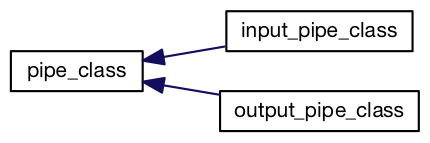
\includegraphics{./img/pipe_class.png}
\caption{Диаграмма классов каналов ввода/вывода}
\label{pipe_class}
\end{figure}
\FloatBarrier

Перенаправление потоков ввода/вывода определяется двумя классами - input\_pipe\_class и output\_pipe\_class. Они принимают векторы начальных и конечных точек соединения соответственно. Начальные точки соединения определяются потомками класса input\_buffer\_class. Конечные – output\_buffer\_class. Точки могут соединять с файлами, а так же с потоками ввода/вывода. Так, например, класс handle\_buffer\_class отвечает за запись и чтение в заданные дескрипторы, будь то дескрипторы консоли или дескрипторы файла.
\FloatBarrier 
\begin{figure}[htb]
\centering
\includegraphics{./img/buffer_class.png}
\caption{Диаграмма классов буфферов}
\label{buffer_class}
\end{figure}
\begin{figure}[htb]
\centering
\includegraphics{./img/runner_class.png}
\caption{Диаграмма классов исполнителей}
\label{runner_class}
\end{figure}
\FloatBarrier
Создание процесса происходит вызовом соответствующей функции у объекта-потомка класса runner – процесс может быть создан синхронно(run\_process) и асинхронно(run\_process\_async). В зависимости от класса(secure\_runner, delegate\_runner, delegate\_instance\_runner) выбирается способ запуска программы. Изначально процесс создается в “замороженном” состоянии. В случае ошибки создания процесса - устанавливается соответствующий статус. После этого процесс запускается. В случае обычного запуска функция возвращает только когда выполнение процесса завершено или случилась какая-либо ошибка. В случае асинхронного запуска функция возвращает сразу – выполнение процедуры запуска происходит в отдельном потоке. 
Информацию о статусе выполнения можно получить вызовом метода get\_process\_status(). В том случае, если программа не завершилась – статус будет иметь значение process\_still\_active.

\subsection{Модули и алгоритмы}

Spawner, являясь модулем автоматизированной системы CATS, в свою очередь разделен на несколько подмодулей — статическая библиотека libspawner, сам spawner или sp, представляющий из себя консольную утилиту, а так же модуль совместимости. Помимо этого в проекте содержится модуль тестирования.

\subsubsection{Библиотека libspawner}

Исходные файлы библиотеки располагаются в соответствующей директории.
В папке inc - содержатся заголовочные файлы. В корне директории находится файл spawner.h, который является основным, для включения в какой-либо проект.

Содержимое папки inc
\begin{itemize}
  \item buffer.h – модуль отвечающий за конечные точки перенаправленных потоков ввода/вывода
  \item compatibility.h – модуль отвечающий за совместимость со старой версией Spawner'а
  \item delegate.h – модуль отвечающий за делегированный запуск процессов
  \item error.h – модуль отвечающий за обработку ошибок системы Spawner а так же за дальнейший их вывод
  \item options.h - модуль отвечающий за класс настроек
  \item pipes.h - модуль отвечающий за перенаправление потоков ввода/вывода
  \item platform.h - модуль отвечающий за системно зависимые переменные и типы
  \item report.h - модуль для получения строковых значений из перечислимых типов проекта
  \item restrictions.h - модуль класса ограничений
  \item runner.h – модуль содержащий базовый и минимальный класс, способный запускать программы
  \item securerunner.h – модуль отвечающий за ограниченный запуск программ
  \item session.h – модуль отвечающий за уникальность сессии делегированного запуска
  \item status.h - модуль статусов
  \item uconvert.h - модуль преобразования единиц, созданный для повышения комфорта работы с программой
\end{itemize}
\FloatBarrier 
\begin{figure}[htb]
\centering
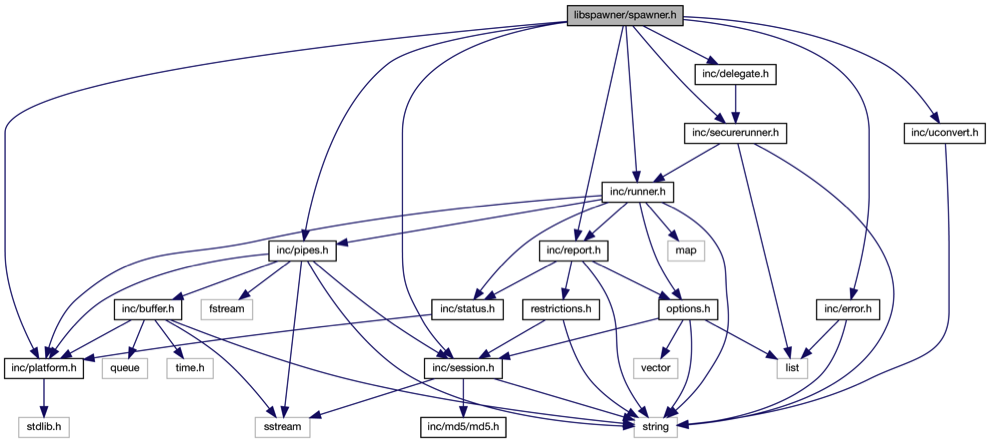
\includegraphics{./img/libspawner.png}
\caption{Схема связи модулей библиотеки libspawner}
\label{libspawner}
\end{figure}
В папке src, в корне или в соответствующей операционной системе директории содержатся реализации соответствующих классов.

Используя набор предоставляемых классов и интерфейсов, можно создавать множество процессов и, контролируя их исполнение, обеспечивать их взаимосвязь друг с другом.

В качестве примера был создан демонстрационный проект(см. материалы в конце), представляющий из себя игру с угадыванием последовательности чисел. После того как программно задаются участники – некоторые исполняемые файлы, программа-исполнитель загадывает последовательность чисел и на догадки программ-участников отвечает сколько из чисел угаданы верно. Игра продолжается, до тех пор, пока все участники не угадают загаданную последовательность чисел. Коммуникация между игроками и исполнителем осуществляется через потоки ввода/вывода, соединенные друг с другом программно, с помощью средств libspawner, а так же подобная программа была реализована с использованием консольного интерфейса Spawner'а.
\FloatBarrier

\subsubsection{Модуль консольной утилиты}
\FloatBarrier 
\begin{figure}[htb]
\centering
\includegraphics[width=\textwidth,keepaspectratio]{./img/utility.png}
\caption{Схема связи модулей консольной утилиты}
\label{utility}
\end{figure}

Проект включает в себя статическую библиотеку libspawner.
Состоит из двух внутренних модулей - модуль парсинга консольных аргументов SimpleOpt и главный модуль, использующий интерфейсы libspawner для реализации поставленной темой задачи.
\FloatBarrier
\subsubsection{Модуль совместимости}
Представляет собой прослойку, позволяющую структуры данных получаемых от библиотеки переводить в различные форматы соответствующие 
\subsubsection{Модуль тестирования}
Содержит набор тестов. Подробнее смотри раздел «Реализация и тестирование».
\subsubsection{Механизм ограничения}
В новой реализации Spawner унаследовал способ наложения ограничений на дочерние процессы. Для этого используется используется механизм JOB\_OBJECT'ов\cite{job_object}, позволяющий на уровне системы контролировать использование системных ресурсов программой, которой был назначен этот объект. В случае превышения конкретного ресурса, можно определить что это был за ресурс и каково было его использование. На некоторые ресурсы ограничения можно накладывать непосредственно. Ресурсы для которых такой возможности нет предлагается наблюдать в отдельном потоке Spawner'а, и, в случае нарушения, завершать JOB\_OBJECT c указанным кодом.

\subsubsection{Механизм перенаправления потоков ввода/вывода}
В данной работе использовался подход, сходный с реализованным в оригинальной версии Spawner'а. Был реализован гибкий интерфейс классов, построенный поверх системной прослойки для осуществления таких схем как «один  источник – много выходов». Интерфейс классов представлен двумя базовыми объектами – соединительный канал (pipe) и буфер данных. Соединительный канал осуществляет связь между соответствующим потоком ввода/вывода дочернего процесса и буфером. Буфер данных представляет собой абстрактный объект, который может осуществлять как запись/чтение файла, консоли, так и работу с участками памяти. Т.е. данные из соединительного канала с помощью объекта буфера могут быть выведены в совершенно различные источники. Каждый объект соединительного канала имеет свой отдельный программный поток, в котором в зависимости от направления канала происходит чтение из буферов и запись или наоборот, чтение из канала и запись в объекты буферов.

\subsubsection{Отключение диалогов об ошибках и пользовательского интерфейса}
Одним из требований к модули была возможность отключение сообщений об ошибках, выдаваемых как средой разработки так и операционной системой. Для решения проблемы были использованные специальные функции WinAPI, такие как SetErrorMode, а так же были установлены специальные параметры при создании дочерних процессов.
Возможность скрытия графического интерфейса также реализуется при помощи создания процесса со специальными параметрами STARTF\_USESHOWWINDOW и SW\_HIDE.

Среда разработки Microsoft Visual Studio при компиляции программ в режиме отладки в случае исключения генерирует диалог об ошибке, которые невозможно скрыть ни одним из указанных выше методом. Для решения этой проблемы использовался запуск контролируемого процесса в режиме отладки и постоянная проверка на исключение. Когда оно возникает Spawner просто завершает дочерний процесс.

\subsubsection{Запуск программ от другого пользователя}
В изначально версии Spawner'а, а так же в некоторых других подобных модулях для запуска процесса от учетной записи другого пользователя использовалась стандартная функция WinAPI CreateProcessWithLogon. Однако, при выполнении этой функции для дочернего процесса автоматически создается анонимный JOB\_OBJECT. Таким образом, в следствие невозможности назначения нескольких таких объектов одной программе получается, что установление ограничений не представляется возможным. В рамках данной работы было проведено исследование и выделено несколько возможных путей решения.

Первый путь решения предполагает собой написания драйвера ядра с использованием недокументированного API (5). В низкоуровневом системном Windows Driver API существует функция ObReferenceObjectByHandle, позволяющая получить доступ ко всем дескрипторам выбранного процесса. Однако, сложность данного решения заключается как в написании подобного драйвера ядра, так и портировании его на другие системы.

Другим решением является запуск процесса-агента. Однако данное решение было признано неподходящим, вследствие необходимости запуска сервиса-агента, постоянно запущенной пользовательской сессии, а так же сложностями с контролируемым исполнением.

Еще одним решением является делегированный запуск. Делегированный запуск представляет собой запуск дочерним процессом еще одного Spawner'а от учетной записи другого пользователя. Этому процессу «делегируется» роль исполнения конечной программы. Ограничения по системным ресурсам создаются в именном объекте JOB\_OBJECT в главном процессе Spawner'а. В роли имени JOB\_OBJECT'а выступает некоторый идентификатор, получаемый исходя из следующих пунктов:
\begin{itemize}
  \item Время запуска родительского процесса Spawner'a
  \item Опции запуска дочернего процесса
  \item Порядковый номер в случае множественного исполнения
\end{itemize}
Полученный идентификатор передаются делегату с помощью внутреннего аргумента -- - -session=<id>.

Однако существует сложность наследования дочерними процессами родительского JOB\_OBJECT'а. Эта сложность решается недокументированным поведением API. Для этого родительскому Spawner'у назначается JOB\_OBJECT с параметрами, запрещающими выход дочерних процессов из него. После этого при создании дочерних процессов под другим пользователям они не получают свой анонимный JOB\_OBJECT, наследуя вместо этого соответствующий объект JOB\_OBJECT родителя. После Затем в родительском процессе отменяется запрет на выход дочерних процессов из JOB\_OBJECT'а и делегированный процесс уже запускает заданную программу с необходимыми опциями.
В рамках данной работы была реализована система перенаправления потоков ввода/вывода, основанная на именных соединительных каналах. Однако, из-за этого некоторые программы не исполнялись корректно. Поэтому было решено реализовать перенаправления на основе стандартных безымянных каналов. Созданные каналы передаются процессу «делегату» в качестве стандартных потоков ввода/вывода при создании. После чего, процесс «делегат» уже передает эти потоки запускаемому дочернему процессу.
В случае если отключен режим отладки (см. подробнее раздыл о скрывании ошибок), процесс «делегат» завершается. Иначе он работает в качестве отладчика. Здесь возникает проблема нотификации главного процесса о том, что в дочернем процессе произошло исключение. Одним из возможных способов реализации является использование системы сообщений JOB\_OBJECT'а.

\subsubsection{Множественное исполнение}
Благодаря гибкой системе соединительных каналов и буферов (см. соответствующий пункт о перенаправлении потоков ввода/вывода), соединение двух каналов возможно с помощью объекта буфера, работающего с памятью как на чтение так и на запись.

\subsubsection{Ограничение по времени простоя}
В рамках данной работы для совместимости, а так же улучшения было принято решение реализовать ограничение по времени простоя. Подобное ограничение успешно используется на Полуфинальном этапе чемпионата АСМ\cite{pcms2}.

Благодаря  этому ограничению можно сэкономить значительное время на уничтожении процессов по факту не выполняющих полезной работы определенное время. Причинами такого поведения программ могут быть: ожидание выполнения операции ввода/вывода, системная операция сна, различные ожидания объектов и пр. Если в старой версии Spawner'а требовалось ждать 10 секунд глобального таймаута, что для 100 тестов является довольно продолжительным, то сейчас подобные ничего не делающие программы могут быть уничтожены за гораздо более короткое время. 
В качестве входных параметров принимается уровень пороговый загрузки, который будет считаться за простой и ограничение на время простоя. Когда уровень загрузки опускается ниже порога, запускается глобальный таймер, по истечении которого дочерний процесс уничтожается с помощью механизма JOB\_OBJECT'ов с соответствующим кодом.


\subsection{Стандарт кодирования}

За основу стиля наименования классов, методов, свойств, функций, типов и т.д. был взят стиль стандартной библиотеки C/C++. Некоторая часть имен использует стиль WinAPI, вследствие специфики.
\iffalse OLD:
Стандарт кодирования описан в документации проекта\cite{codingstyle}:
\begin{itemize}
  \item Ключевые слова пишутся маленькими буквами.
  \item Символы табуляции запрещены.
  \item Не следует отделять операции, запятые точку с запятой и скобки пробелами.
  \item Размер отступов: два пробела для каждого уровня отступа.
  \item Перед блоком begin ... end следует делать отступы.
  \item Не вложенные подпрограммы разделяют двумя пустыми строчками.
  \item Вложенные подпрограммы отделяются одним пробелом.
  \item Однострочные условные операторы запрещены. Условие и действие нужно писать на разных строчках.
  \item У идущих подряд условных операторов следует писать else и последующее if 
    на одной строке.
  \item Идентификаторы подпрограмм, состоящие из нескольких слов необходимо писать
    маленькими буквами, разделяя слова символом подчёркивания.
  \item Идентификаторы переменных и типов, состоящие из нескольких слов следует писать
    маленькими буквами слитно без разделительных символов.
\end{itemize}
\fi

\section{Реализация и тестирование}

Работоспособность системы была проверена на следующих системах
\begin{itemize}

  \item Windows 7 x64
  \item Windows Server 2008 x86
  \item Windows XP SP3 x86
\end{itemize}
И на следующих компиляторах
\begin{itemize}
  \item Microsoft Visual Studio 2008 x86
  \item Microsoft Visual Studio 2012 x86
  \item Microsoft Visual Studio 2012 x64
  \item MinGW GCC 4.7.7
\end{itemize}
Для наибольшей совместимости рекомендуется использовать компилятор GCC.

В рамках данной работы, для облегчения проверки основных механизмов работы на корректность на разных системах была разработана система тестирования.

Для разработки данной системы был использован язык Perl и его стандартная библиотека тестирования. Для сборки тестов была написана серия шаблонов CMake файлов, позволяющих создавать иерархию в тестовых директориях не усложняя при этом процесс сборки. Так же данные шаблоны автоматически копируют получившиеся исполняемые файлы тестов для дальнейшей работы с ними.
Конкретный тест представляет собой исполнение тестовой программы при помощи модуля Spawner, получение отчета исполнения и, наконец, проверки соответствующих полей. Так как в модуле judge системы CATS существует реализация процедуры запуска Spawner'a и разбора отчета, было принято решение использовать для написания системы тестирования язык Perl и вынести общие процедуры в отдельный модуль.
Тесты разбиваются по категориям и разносятся по соответствующим папкам, представляющим собой отдельную директорию с модулем тестирования и набором проектов. В каждый проект входит отдельные исходники на каком-либо языке программирования, а так же файл тестов. Библиотека тестирования имеет составляющую, написанную на CMake, а так же составляющую, написанную на Perl. Часть на CMake используется исключительно для сборки и ,поэтому, проводится в первую очередь. После того как все тестовые программы были успешно собраны и перенесены в общую директорию можно запускать основной скрипт Perl, который запустит все добавленные тесты.
Один из наборов тестов представляет собой проверку контроля исполнения старой версии и новой Spawner'а на идентичность в некотором приближении на наборе простых программ.

Так же присутствуют тесты на проверку каждых ограничений и опций в отдельности.
Общее количество тестов - около 40. 
Было проведено внедрение модуля в систему CATS и он прошел тестирование в реальных условиях нескольких соревнований, таких как Четвертьфинал командного чемпионата АСМ, а так же школьные олимпиады по программированию. Работа модуля сопровождалась переменным успехом, однако выявленные в ходе проверки ошибки и несовместимости были или будут исправлены. Помимо этого тестирование модуля осуществлялось вручную по методу белого ящика на нескольких операционных системах и средах разработки.


\pagebreak

\section*{Заключение}
\addcontentsline{toc}{section}{Заключение}

В ходе дипломной работы был расширен модуль контроля исполнения программ. Были реализованы в полном объеме поставленные функциональные требования.
Так же разработанный модуль был введен в состав системы CATS на место старой версии, а в саму систему были внесены изменения для более тесной интеграции. 

Основная программа состоит из двух частей — своих исходников и библиотеки libspawner. Объём кода составляет 250KB (5088 строк).
В ходе предквалификационной практической работы были изучены: модуль judge системы CATS, система сборки CMake, язык программирования Perl.

Так же были углублены знания в WinApi и Microsoft Windows.
По имеющимся на данный момент результатам можно говорить об успешной реализации подмножества функциональных требований.

\pagebreak

%\bibliography{biblio}     %% имя библиографической базы (bib-файла) 
\begin{thebibliography}{99}
\bibitem{acm} Международная студенческая олимпиада по программированию ACM/ICPC --- Wikipedia
\bibitem{prog_challenges} Steven S Skiena, Miguel A. Revilla, Programming Challenges: The Programming Contest Training Manual, 2002
\bibitem{cats} Система организации соревнований по программированию \url{http://imcs.dvfu.ru/cats}
\bibitem{rozhkov} Рожков М., Кленин А.С. Дипломная работа «Система автоматического тестирования программ и организации соревнований по программированию». --- ДВГУ, 2004г.
\bibitem{matvienko} Матвиенко В., Кленин А.С.Курсовая работа «Рендеринг математических выражений в MathML и HTML». --- ДВГУ, 2005г.
\bibitem{konovalova} Коновалова Д., Кленин А.С. Курсовая работа «Поиск сходных алгоритмических конструкций в программном коде». --- ДВГУ, 2005г.
\bibitem{perepechin} Перепечин В.В., Кленин А.С. Курсовая работа «AJAX-интерфейс для системы CATS». --- ДВГУ, 2007г.
\bibitem{tuphanov} Туфанов И.Е., Кленин А.С. Курсовая работа «Универсальный генератор тестов для системы CATS». --- ДВГУ, 2008г.
\bibitem{khrapchenkov} Храпченков П.Ф., Кленин А.С. Курсовая работа «Модуль контролируемого исполнения программ Spawner». --- ДВФУ, 2013г.
\bibitem{sandboxing_def} Vassilis Prevelakis, Diomidis Spinellis «Sandboxing Applications», 2001
\bibitem{prototype} Модуль контролируемого исполнения программ Spawner, предыдущая версия \url{http://imcs.dvgu.ru/cats/docs/spawner.html}
\bibitem{vseros} Всероссийская олимпиада школьников --- Методические рекомендации. \url{http://rosolymp.ru/index.php?option=com_content&view=article&id=6451&Itemid=909}
\bibitem{virtualization} Виртуализация: технологические подходы \url{http://www.pcmag.ru/solutions/detail.php?ID=34643}
\bibitem{seccomp} [PATCH] seccomp: secure computing support \url{http://git.kernel.org/cgit/linux/kernel/git/tglx/history.git/commit/?id=d949d0ec9c601f2b148bed3cdb5f87c052968554}
\bibitem{ejudge} Система проведения соревнований EJudge \url{http://ejudge.ru/}
\bibitem{pcms2} Модуль контролируемого исполнения программ PCMS2 \url{http://neerc.ifmo.ru/trains/information/software.html}
\bibitem{contester} Система для проведения турниров и индивидуального решения задач по олимпиадному программированию \url{http://www.contester.ru/}
\bibitem{executor} Автоматизированная сетевая тестирующая система для проведения турниров по программированию по правилам ACM \url{http://acmtest.ru/}
\bibitem{pccs} PC$^2$(Programming Contest Control System) \url{http://www.ecs.csus.edu/pc2/}
\bibitem{olympiads} Олимпиады по программированию \url{http://olympiads.ru/school/system
/index.shtml}
\bibitem{domjudge} Автоматизированная тестирующая система, для проведения соревнований по программированию \url{http://domjudge.sourceforge.net/}
\bibitem{dudge} Универсальная система для проведения олимпиад по программированию \url{http://code.google.com/p/dudge/}
\bibitem{spawner_src} Модуль контролируемого исполнения программ Spawner \url{https://github.com/ShigiDono/Spawner}
\bibitem{gpl} Free Software Foundation, Inc. GNU General Public License. \url{http://www.gnu.org/licenses/gpl.html}. - 2007г.
\bibitem{job_object} Официальный сайт MSDN. Статья о JOB\_OBJECT. \url{http://msdn.microsoft.com/en-us/library/windows/desktop/ms684161\%28v=vs.85\%29.aspx}

  

  
\end{thebibliography}
\addcontentsline{toc}{section}{Список литературы}

\pagebreak

\noindent Автор работы \superunder{\hrulefill}{\hspace{2cm}(подпись)\hspace{2cm}} (Ф.И.О.)\\

\noindent{}Квалификационная работа допущена к защите\\

\noindent{}Назначен рецензент\\
\superunder{\hrulefill}{(Фамилия, И.О. рецензента, ученая степень, ученое звание)\hspace{5cm}}\\

\vspace{2\baselineskip}
\noindent\begin{tabular}{p{0.5\textwidth} p{0.45\textwidth}}
\parbox{8cm}{Зав. кафедрой информатики,\\ математического и компьютерного\\ моделирования} &
\hfill А.~Ю.~Чеботарев\\
\end{tabular}
\vspace{2\baselineskip}
\begin{flushright}
Дата <<\rule{1cm}{0.5pt}>>\rule{3cm}{0.5pt}\quad 2014 г.
\end{flushright}

\end{document}
%
%
%
%
%
%
%
%
%
%
%
%
%